\documentclass[12pt]{article}
\usepackage{natbib}
\usepackage{eso-pic}
\usepackage{amsmath} % flere matematikkommandoer
\usepackage{amssymb}
\usepackage[utf8]{inputenc} % æøå
\usepackage[T1]{fontenc} % mere æøå
\usepackage[danish]{babel} % orddeling
\usepackage{verbatim} % så man kan skrive ren tekst
\usepackage[a4paper, margin = 1in]{geometry}
\usepackage{graphicx}
\usepackage{booktabs}
\usepackage{enumitem}
\usepackage{placeins}
\usepackage{hyperref}
\usepackage{tocbibind}

\author{
  Christian Kjær Larsen\\
  \texttt{011292} \\[.4cm]
  Lukas Svarre Engedal\\
  \texttt{210790} \\[.4cm]
  Tobias Sønderskov Hansen\\
  \texttt{240395} \\[.4cm]
  Instruktor: Aske Mottelson\\[.4cm]
  \vspace{10cm}
}

\title{
  \vspace{3cm}
  \Huge{ProjDat 2015} \\[.25cm]
  \large{Delrapport 2}
}

\begin{document}

\AddToShipoutPicture*{\put(0,0){\includegraphics*[viewport=0 0 700 600]{includes/nat-farve}}}
\AddToShipoutPicture*{\put(0,602){\includegraphics*[viewport=0 600 700 1600]{includes/nat-farve}}}

%% Change `ku-en` to `nat-en` to use the `Faculty of Science` header
\AddToShipoutPicture*{\put(0,0){\includegraphics*{includes/nat-en}}}

\clearpage\maketitle
\thispagestyle{empty}

\newpage

\tableofcontents

\thispagestyle{empty}

\newpage
\pagestyle{plain}
\setcounter{page}{1}
\pagenumbering{arabic}

\section{Review}
\subsection{Designing for usability: key principles and what designers think}
\label{sub:designing_for_usability}
\paragraph{Referat}
Artiklen \cite{gould1985designing} beskriver en overordnet metode til design og udvikling af brugervenlige systemer. Denne tilgangsvinkel består af 3 grundlæggende principper: tidligt fokus på brugerne, empiriske målinger og iterativt design. Artiklen tager udgangspunkt i udviklingen af IBM's \emph{Audio Distribution System} (ADS) hvor disse principper blev anvendt.

Ved første princip påstås at det er nødvendigt for systemudviklerne fra starten at sætte sig ind i hvem systemets tiltænkte målgruppe er. Metoden anbefaler at udviklerne danner sig en \emph{forståelse} for brugerne, frem for blot at lave en karakterisering. Udover selve brugerne, skal udviklerne også sætte sig ind i hvilken sammenhæng systemet skal bruges og hvilke opgaver det skal løse, samt hvordan et evt. nuværende system løser disse opgaver.

Andet princip, \emph{empiriske målinger}, beskriver brugen af prototyper og simulationer til at teste mod målgruppen for at studere dennes reaktion. Personer der selv har været med til at udvikle systemet vil næsten uundgåeligt anvende systemet anderledes end en typisk bruger, derfor er det vigtigt at systemet også bliver afprøvet af målgruppen, og at målgruppens respons bruges i den efterfølgende udvikling.

\emph{Iterativt design} går ud på at de problemer der opdages under afprøvningen skal løses. Dette sikres ved at opdele systemudviklingen i en masse gentagelser af design og afprøvning, hvor resultaterne af afprøvningen i én iteration påvirker deisgnet i den næste. Dette er i kontrast til mere lineære modeller, hvor der i stedet udarbejdes en detaljeret kravspecifikation, og en egentlig afprøvning først sker til sidst i projektet.

Når udviklere præsenteres for disse principper er reaktionen typisk at det virker meget intuitivt og mange påstår at de allerede anvender disse principper. Ifølge undersøgelser foretaget af folkene bag metoden tyder det dog på, at der er forskel på hvad systemudviklerne selv siger de gør, og hvad de egentlig gør i praksis.

\paragraph{Perspektivering}
De tre principper fra artiklen indgår alle i et vist omfang i systemudviklingsmetoden præsenteret i OOSE.

Med hensyn til tidligt fokus på brugerne, så inkorporerer OOSE's fremgangsmåde bl.a. dette i form af en \emph{requirements elicitation}, der beskriver de forskelllige typer brugere og i hvilke sammenhænge de systemet anvendes.

Artiklen understreger vigtigheden af at kunne foretage ændringer baseret på brugernes reaktioner, derfor er det vigtigt at systemet er struktureret på en måde der tager højde for dette. Man kan sammenligne dette med \emph{Entity-Boundary-Control} fremgangsmåden beskrevet i OOSE, der fokuserer på at opdele systemet i nogle forholdsvis uafhængige elementer, så der eksempelvis kan ændres i brugergrænsefladen uden at det påvirker resten af programmet.

Både metoden beskrevet i artiklen og de fremgangsmåder præsenteret i OOSE er agile. Den grundlæggende metode er altså fælles for dem alle, udviklingen sker i iterationer af henholdsvis design og brugertest.

\subsection{A Rational Design Process: How and Why to Fake It}
\label{sub:a_rational_design_process}
\paragraph{Referat}
I artiklen \cite{parnas1986rational} prøver forfatterne at beskrive en ideel udviklingsproces og den dokumentation der kræves. Hovedargumentet i artiklen er dog, at selvom man ikke har fuldt grundlag for en altomfattende kravspecifikation, så skal man stadig producere dokumentation som hvis man havde.

Derfor mener forfatterne, at hvis man ikke har en helt beskrivende kravspecifikation, så er det vigtigt at kende processen, så man som udvikler kan hjælpe designerne med, at finde de manglende informationer. Det gør, at man tidligere i processen kan få fundet fejl i designet, så de ikke kommer med i det endelige system.

Den metode som Parnas og Clements foreslår i artiklen er, at man starter med at dokumentere krav. Dette er med til at gøre det lettere at estimere tidsforbruget, blive klog på problemområdet for alle involverede og hjælpe med ting som test, inkonsistens og udskiftning af personer, da den specifikke viden er skrevet ned.

Derefter mener de, at man skal nebryde arbejdet i moduler, så det kan uddelegeres til forskellige udviklere. Grænsefladerne mellem modulerne og selve kravene til modulerne dokumenteres grundigt. Til sidst produceres kildekoden, og produktet er klart. Der argumenteres for, at hvis alt forarbejdet er gjort grundigt, så er programmeringen ligetil.

Hele titlen på artiklen, det at \emph{fake} den ideelle udviklingsproces går ud på, at hvis man følger den ideelle proces, så når man mangler et stykke information, så noterer man dette i designdokumentationen. Når man så finder de rigtige svar senere, så rettes dokumentationen hele vejen ned i kæden. Dette skulle så meget gerne producere en korrekt specifikation i sidste ende.

\paragraph{Perspektivering}
Den idealiserede udviklingsproces som beskrives i \cite{parnas1986rational} har mange ting til fælles med nogle af kapitlerne i \cite{OOSE}. Den i artiklen omtalte kravspecifikation har mange ting til fælles med det i bogen omtalte \emph{Requirement Analysis Document} (Kapitel 4). I begge dokumenter indgår alle informationer, der skal til at udvilkle systemet.

I artiklen beskrives hvordan dette dokument kan bruges til at nedbryde problemet i moduler som kan takles af mange forskellige udviklere. Det er også hvad der foreslås i kapitel 6 i \cite{OOSE}. Her nedbrydes systemet efter analysemodellen som er resultatet af kravspecifikationen. Det er også her, ligesom i artiklen, at grænsefladerne mellem modulerne specificieres, så en udvikler nemt og fejlfrit kan udvikle delsystemet. I artiklen argumenterer forfatterne for, at for hvert delsystem, så skal der fremstilles en kravspecifikation med samme struktur som for hele systemet. Det bliver en slags rekursiv dokumentation, da et delsystem godt kan bestå af flere. Fra et ledelsesperspektiv er det beskrevet i kapitel 14 i \cite{OOSE} hvordan denne nedbrydning uddelegeres mellem udviklere, så arbejdet foregår mest effektivt.

Artiklen omtaler processen som ideel. Den omtalte proces er i praksis det vi kender som \emph{waterfall}-modellen. I mere moderne softwareudvikling stiller man spørgsmålstegn ved, om det er den optimale proces. Det er især efter udbredelsen af agile metoder som \emph{SCRUM} \cite{sutherland2010jeff} og andre. Her erkender man, at det er nærmest umuligt at designe software på samme måde som man designer broer på, da der simpelthen er for mange ukendte når man starter. Dette udbedres så ved at beskrive kravene samtidig med at systemet udviklet, da det så er nennere at finde fejl i designet undervejs.

\newpage
\section{Abstract}
\label{sec:abstract}
Our project is about developing an e-learning system for use in the newly created introductory computer science course at the Institute of Computer Science at Copenhagen University, called \emph{Programmering og Problemløsning}. Our clients are Martin Dybdal and Oleksandr Shturmov, both employed at the institute, who will be in charge of the course. In the course, the students will be taught the \verb!F#! language.

The aim of the e-learning system is to introduce new students to programming in a simple and user-friendly way, and to teach them various basic ideas and concepts in programming in general and \verb!F#! in particular. This is done by presenting the students with an array of different exercises, which are sorted based on subject and difficulty, and presented to students in a specific and meaningful order.

The system will have two different kinds of users: students and admins.

Students will mainly be working on the various exercises, and they will also be able to get hints for the exercises if needed and provide feedback on the exercises and hints once completed. Students should also be able to see how well they are doing so far, for instance how many of the exercises belonging to a particular subject matter they have solved.

The primary role of the admins will be managing the exercises and supervising how well the students are doing. They should be able to easily delete or modify existing exercises or add new ones, as well as manage the order in which the students are presented with the exercises. They should also be able to get various statistics about how the students are doing in order to improve and optimize the exercises, their order and their subjects.

\section{Formål og rammer}
\label{sec:formal_og_rammer}
I dette afsnit beskrives systemets formål og rammer ved \textit{FACTOR}-kriteriet.
\begin{description}
    \item[Funktionalitet]
        Besvare og oprette programmeringsspørgsmål, Analysere de studerendes fremskridt.
    \item[Anvendelsesområde]
        Loginsystem, Spørgsmålshåndtering, Spørgsmålsbesvarelse, Analyse.
    \item[Betingelser]
        Undervisere har begrænsede resurser. Studerende har svært ved programmering.
    \item[Teknologi]
        Webapplikation med teknologi der er nemt at sætte sig ind i.
    \item[Objekter]
        Studerende, Spørgsmål, Hints, Undervisere.
    \item[Ansvar]
        E-læringssystem til hjælp af studerende med programmering.
\end{description}
\section{Kravspecifikation}
\label{sec:kravspecifikation}

\subsection{Krav}
\label{sub:krav}
\paragraph{Funktionelle krav}
De funktionelle krav for systemet er i tråd med afsnit 4.3.1 i \cite{OOSE}, nemlig at de omhandler den specifikke brug af systemet.
\begin{itemize}
    \item Systemet skal være en hjemmeside med opgaver, som kan løses individuelt af studerende.
    \item Der kræves login, så man kan følge med i den studerendes udvikling.
    \item Spørgsmålene skal være grupperede efter hvilke læringsmål de tester.
    \item Læringsmålene skal igen grupperes i nogle blokke, hvor idéen så er at man gennemgår blokkene én af gangen i en bestemt rækkefølge, og at sværhedsgraden stiger løbende.
    \item Der skal være hints til opgaverne som de studerende kan benytte hvis nødvendigt, og de studerende skal så kunne give feedback til hints'ne.
    \item Alle forsøg på opgavebesvarelser skal gemmes i en log.
\end{itemize}
Hvis der er tid i en af de senere iterationer, så er der en række ekstra krav som kan implementeres.
\begin{itemize}
    \item Loggen skal bruges til at give underviseren information om hvilke spørgsmål der er svære.
    \item Der skal tilføjes en grad af \emph{gamification}, så der gives badges og point for fremskridt, og det bliver muligt at følge med i andres fremskridt.
    \item Hvis man ikke har øvet sig i et emne i et stykke tid, så falder ens erfaring i området.
\end{itemize}

\paragraph{Ikke-funktionelle krav}
\label{par:ikke_funktionelle_krav}
I afsnit 4.3.2 i \cite{OOSE} beskrives ikke-funktionelle krav som krav, der ikke direkte beskriver funktionaliteten, men mere generelle krav omkring ting som brugervenlighed, ydeevne, pålidelighed og hvor vedligeholdesesvenligt systemet er.

De ikke-funktionelle krav til dette projekt er forholdsvis begrænsede, idet vi har fået ret stor frihed i forhold til hvordan vi løser opgaven af vores kunde.

\begin{itemize}
\item Det skal være nemt at tilføje nye opgaver til systemet, sådan at kursuslederne efterfølgende kan opbygge en tilstrækkelig samling af opgaver til de studerende.
\item Det endelige produkt skal gerne skal være så simpelt og modulært som muligt, sådan at det er nemt at overtage, udvide og bygge videre på efter at vi overgiver projektet til kunden.
\item Ingen af kunderne er web-udviklere, så det er også vigtigt at det valgte framework er veldokumenteret og rimeligt simpelt at bruge.
\end{itemize}

\subsection{Use case model}
\label{sub:use_case_model}
\begin{figure}[htpb]
  \centering
  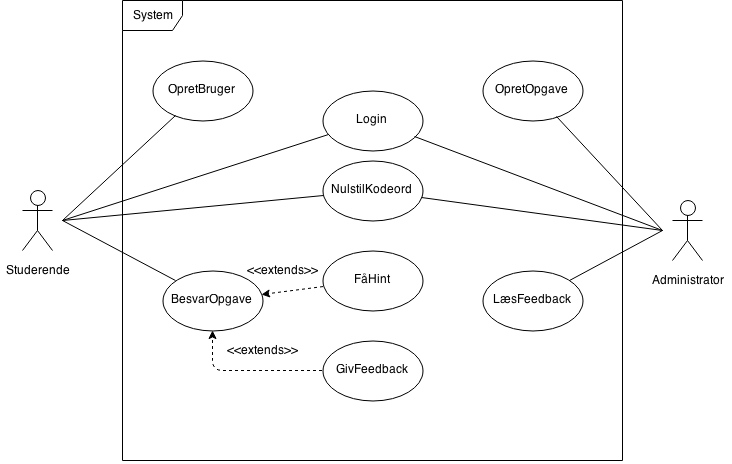
\includegraphics[width=0.8\linewidth]{figures/UseCaseModel.png}
  \caption{Use case model for vores system.}
  \label{fig:use_case_model}
\end{figure}
På Figur \ref{fig:use_case_model} kan man se vores use case model diagram. Vi har at gøre med to aktører, nemlig studerende og administratorer. Det vigtige for studerende er at de kan oprette sig på siden, og at de har adgang til opgaver de kan besvare. Det vigtige for administratorer er at de kan administrere opgaverne, og at de kan få feedback og statistik på hvordan de studerende klarer opgaverne. Begge aktører skal desuden kunne benytte simpel funktionalitet i forbindelse med deres login.

\subsection{Use cases}
\label{sub:use_cases}
På Figur \ref{fig:use_case1} ses en beskrivelse af use casen, hvor en studerende opretter sin bruger. Det er en simpel use case, der beskriver i detaljer hvordan processen med at oprette sig som bruger i systemet skal foregå.

\begin{figure}[htpb]
    \centering
    \begin{tabular}{r p{10cm}}
        \toprule
        \textit{Navn på use-case:} & \verb!OpretBruger! \\
        \hline
        \textit{Deltagende aktører:} & Påbegyndt af en studerende \\
        \hline
        \textit{Hændelser:} & \begin{enumerate}[nolistsep]
            \item En studerende åbner hjemmesiden og klikker på \verb!register!
            \item Den studerende indtaster sine brugeroplysninger, dvs. ku-id og løsen.
            \item Systemet opretter brugeren, og sender en e-mail med et aktiveringslink.
            \item Den studerende klikker på linket, og kontoen aktiveres.
            \item Den studerende bringes til login-siden.
            \item Den studerende indtaster ku-id og løsen og klikker \verb!Login!
            \item Der informeres om succesfuldt login, og brugeren bringes til applikationen.
        \end{enumerate}  \\
        \hline
        \textit{Startbetingelse:} & En studerende har ingen konto, og er ikke logget ind. \\
        \hline
        \textit{Slutbetingelse:} & En studerende har en aktiveret konto og er logget ind. \\
        \bottomrule
    \end{tabular}
    \caption{Use case omkring opretning af brugere.}
    \label{fig:use_case1}
\end{figure}

På Figur \ref{fig:use_case2} ses en beskrivelse af use casen, hvor en studerende svarer på spørgsmål. Den er på et relativt højt abstraktionsniveau, da vi ikke er helt sikre på hvordan workflowet i systemet er endnu.

\begin{figure}[htpb]
    \centering
    \begin{tabular}{r p{10cm}}
        \toprule
        \textit{Navn på use-case:} & \verb!BesvarOpgave! \\
        \hline
        \textit{Deltagende aktører:} & Påbegyndt af en studerende \\
        \hline
        \textit{Hændelser:} & \begin{enumerate}[nolistsep]
            \item En studerende åbner hjemmesiden.
            \item Vedkommende vælger et emne inden for en læringsblok der er låst op ved at have færdiggjort den forrige.
            \item Systemet præsenterer et spørgsmål for den studerende. Der kan være flere typer spørgsmål (multiple-choice, udfyldning med flere).
            \item Den studerende indtaster et svar.
            \item Systemet giver respons på svaret, og gemmer det i en historik.
            \item Den studerende trykker næste, for at få et spørgsmål mere.
            \item Hvis den studerende har svaret på nok spørgsmål, så kan den studerende vælge en ny kategori.
            \item Den studerende lukker browseren.
        \end{enumerate}  \\
        \hline
        \textit{Startbetingelse:} & En studerende der er logget ind. \\
        \hline
        \textit{Slutbetingelse:} & En studerende der er logget ind og har besvaret en eller flere opgaver. \\
        \bottomrule
    \end{tabular}
    \caption{Use case omkring besvarelse af opgaver.}
    \label{fig:use_case2}
\end{figure}

Et af kravene for systemet er, at det skal være nemt for underviserne i kurset at oprette nye opgaver. Da underviserne selv er dataloger, så vil det være optimalt hvis man kan lave spørgsmålene i et struktureret filformat. Vi har foreslået \verb!YAML!, derfor er use-casen på Figur \ref{fig:use_case3} meget simpel, og består kun af fil-upload.
\begin{figure}[htpb]
    \centering
    \begin{tabular}{r p{10cm}}
        \toprule
        \textit{Navn på use-case:} & \verb!OpretOpgave! \\
        \hline
        \textit{Deltagende aktører:} & Påbegyndt af en administrator \\
        \hline
        \textit{Hændelser:} & \begin{enumerate}[nolistsep]
            \item Vedkommende trykker på \verb!Add Question!.
            \item En YAML fil uploades i en formular.
            \item Brugeres informeres om at spørgsmålet er oprettet.
        \end{enumerate}  \\
        \hline
        \textit{Startbetingelse:} & En administrator der er logget ind. \\
        \hline
        \textit{Slutbetingelse:} & En administrator der er logget ind og har oprettet en opgave. \\
        \bottomrule
    \end{tabular}
    \caption{Use case omkring oprettelse af opgaver.}
    \label{fig:use_case3}
\end{figure}

\subsection{Klassediagram}
\begin{figure}[htpb]
    \centering
    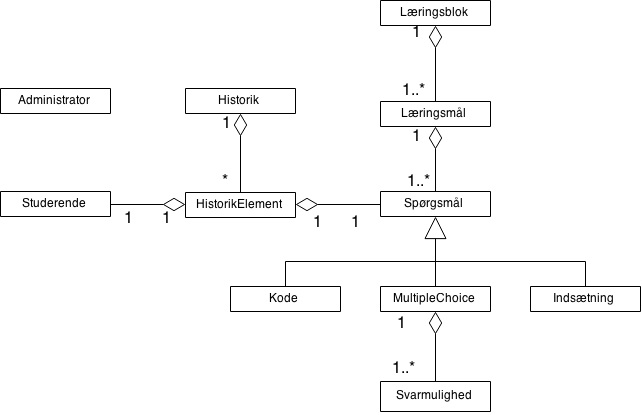
\includegraphics[width=0.8\linewidth]{figures/ClassDiagram.png}
    \caption{Klassediagram af problemområdet}
    \label{fig:class_diagram}
\end{figure}
På Figur \ref{fig:class_diagram} kan man se vores klassediagram. Størstedelen af klasserne har at gøre med opgaverne og deres inddeling i forskellige grupper samt de forskellige typer af opgaver der findes. Derudover er der et par klasser der har at gøre med den log der føres over de studerendes opgavebesvarelser, for at de kursusansvarlige kan følge med i hvad der går godt og mindre godt. Endeligt er der en klasse for studerende og en klasse for administratorne.

\subsection{BCE-model}
\begin{figure}[htpb]
  \centering
  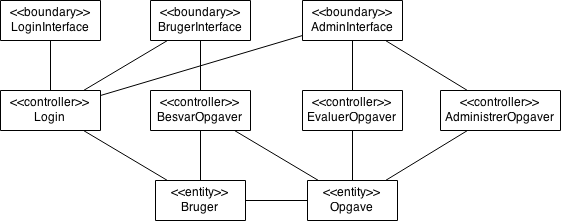
\includegraphics[width=0.8\linewidth]{figures/BCE-Model.png}
  \caption{BCE model for vores system.}
  \label{fig:bce_model}
\end{figure}
På Figur \ref{fig:bce_model} kan man se vores BCE model. Modellen har to entity-objekter, fire controller-objekter samt tre boundary-objekter.

De to entity-objekter er \emph{Bruger} og \emph{Opgave}. \emph{Bruger} indeholder informationer om hver enkelt bruger som login-oplysninger, hvor vidt brugeren er en studerende eller en admin samt hvilke opgaver brugeren allerede har løst. \emph{Opgave} indeholder alle informationerne om de enkelte opgaver, det er både selve opgaven der skal løses samt statistik omkring hvordan det er gået når studerende har løst opgaven.

Modellen har tre boundary-objekter, hvor det første man vil møde når man indlæser siden er \textit{login}-brugergrænsefladen, der sammen med \emph{login}-controlleren sørger for at logge brugerne ind i systemet. Derefter vil man så enten have adgang til \emph{Bruger}-grænsefladen eller \emph{Admin}-grænsefladen afhængig af hvad ens status er, og derfra har man adgang til en række controllers.

Modellen har fire controller-objekter, hvor den første er \emph{login}-controlleren der som tidligere nævnt står for at logge brugere ind i systemet. Som studerende vil man have adgang til \emph{BesvarOpgave}-controlleren, der snakker sammen med \emph{Bruger} og \emph{Opgave} og sørger for at stille brugeren de rigtige opgaver. Som admin vil man have adgang til to controllers, nemlig \emph{EvaluerOpgave}-controlleren og \emph{AdministrerOpgave}-controlleren. \emph{EvaluerOpgave}-controlleren snakker sammen med \emph{Opgave} og giver en adgang til de forskellige slags statistik der bliver samlet om opgaverne, og \emph{AdministrerOpgave}-controlleren snakker ligeledes sammen med \emph{Opgave} og giver en adgang til at slette eller ændre i eksisterende opgaver samt tilføje nye.

\subsection{Sekvens-diagrammer}
\begin{figure}[htpb]
    \centering
    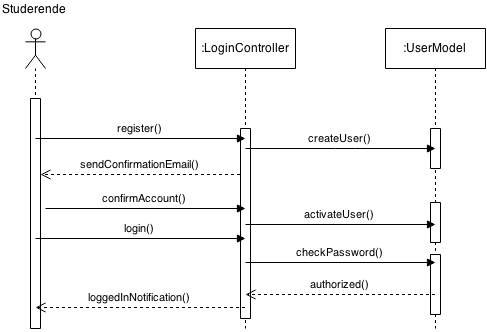
\includegraphics[width=0.7\linewidth]{figures/OpretBrugerUseCase.png}
    \caption{Sekvensdiagram over opretning af bruger}
    \label{fig:opret_bruger_sekvens}
\end{figure}
På Figur \ref{fig:opret_bruger_sekvens} kan man se sekvens-diagrammet for den første use case, der beskriver hvordan en studerende opretter sig som bruger i systemet.

\begin{figure}[htpb]
    \centering
    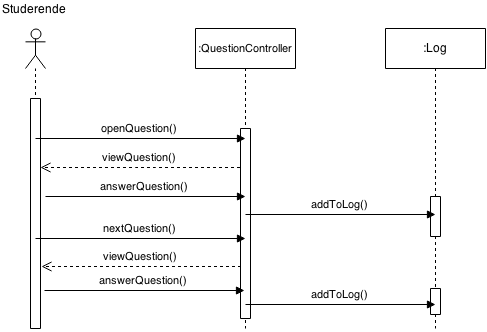
\includegraphics[width=0.7\linewidth]{figures/SvarUseCase.png}
    \caption{Sekvensdiagram over besvarelse af spørgsmål}
    \label{fig:svar_sekvens}
\end{figure}
På Figur \ref{fig:svar_sekvens} kan man se sekvens-diagrammet for den anden use case, der beskriver hvordan en studerende besvarer spørgsmål.

\begin{figure}[htpb]
    \centering
    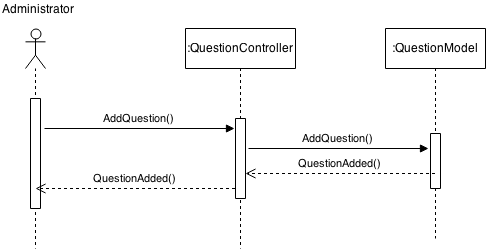
\includegraphics[width=0.7\linewidth]{figures/OpretSporgsmalUseCase.png}
    \caption{Sekvensdiagram over opretning af spørgsmål}
    \label{fig:opret_sp_sekvens}
\end{figure}
På Figur \ref{fig:opret_sp_sekvens} kan man se sekvens-diagrammet for den tredje use case, der beskriver hvordan en administrator opretter et nyt spørgsmål i systemet.

\section{Systemdesign}
\label{sec:systemdesign}
Ikke implementeret

\section{Program- og systemtest}
\label{sec:program_og_systemtest}
Ikke implementeret

\section{Brugergrænseflade og interaktionsdesign}
\label{sec:brugergraenseflade}
Ikke implementeret

\section{Projektsamarbejdet}
\label{sec:projektsamarbejdet}
Siden afleveringen af delrapport 1 har der været påskeferie, eksamensuge og blokferie, og vi er derfor ikke kommet så meget videre med projektet og har derfor heller ikke haft meget kontakt indbyrdes.

Her i blokferien har vi så haft vores andet møde med vores kunder, hvor vi snakkede om diverse aspekter af projektet og diskuterede opbygning og struktur af systemet. Vi er stadig på et stadie i vores diskussion med kunden hvor vi snakker relativt abstrakt om tingene, og vi er også som regel rimelig enige om tingen, og vi har derfor endnu ikke rigtig nået til at punkt hvor vi har følt at det var nødvendigt at tage et grundigt referat af hvad der blev snakket om.

Vi har desuden mødtes to gange i gruppen i blokferien, hvor vi har sat os i kantinen på DIKU for at sammen skrive delrapport 2, og det har fungeret udemærket. Vi har endnu ikke haft nogen deciderede \emph{møder} i gruppen hvor det har været nødvendigt med referat og dokumentation og den slags. Vi kommunikerer stadig på mail både internt i gruppen og med kunden, og vi bruger ligeledes Github til at dele vores arbejde med hinanden og med kunden, og begge dele fungerer også stadig udemærket.

Når vi har afleveret delrapport 2 er det planen at vi så vil mødes i gruppen og konkret diskuterer hvordan vi vil implementere vores system, f.eks. ift. opbygningen af databasen og hjemmesiden, og så sammen starte på at skrive koden. Når vi når dertil kan vi så se hvordan det går med arbejdet og med at dele det op imellem os og kommunikere indbyrdes, og der bliver det måske også mere relevant at dokumentere nogen af de ting vi snakker om i anden form end i delrapporterne.

\newpage
\appendix
\section{Versionsstyring}
Link til github: \url{https://github.com/christiankjaer/pop-webhelp}

\section{Changelog}
\begin{tabular}{l l l}
08-04-2015 & CKL & Dokument oprettet. \\
14-04-2015 & CKL & Tilføjet use cases og krav. \\
16-04-2015 & LSE & Tilføjet UseCaseModel og BCE model. \\
16-04-2015 & CKL & Tilføjet review af Parnas og Clements. \\
17-04-2015 & TSH & Tilføjet review af Gould og Lewis. \\
17-04-2015 & LSE & Tilføjet Abstract og Projektsamarbejdet. \\
17-04-2015 & CKL & Tilføjet use cases, sekvensdiagram og klassediagram. \\
\end{tabular}

\section{Timeline}
\begin{tabular}{l l p{8cm}}
11-03-2015 & Første møde med kunde: & Vi har første møde med kunden hvor vi snakker om hvad projektet går ud på og diskuterer krav og løsningsforslag. \\
16-04-2015 & Andet møde med kunde: & Vi har haft andet møde med kunden, hvor vi har snakket om modellen for de opgaver der skal være i systemet. \\
\end{tabular}

\bibliographystyle{alpha}
\bibliography{refs}{}


\end{document}
